\section{OpenTPOD: Open Toolkit for Painless Object Detection}
\label{sec: app-dev-tpod}

Training a DNN for object detection is not trivial.  In particular, it involves
constructing a correctly-labeled training data set with millions of positive and
negative examples. The training process itself may take days to complete, and
requires a set of arcane procedures to ensure both convergence and efficacy of
the model. Fortunately, one does not typically need to train a DNN from scratch.
Rather, pretrained models based on public image data sets such as ImageNet are
publicly available. Developers can adapt these pretrained models to detect
custom classes for new applications, through a process called \emph{transfer
learning}.  The key assumption of transfer learning is that much of the training
that teaches the model to discover low-level features, such as edges, textures,
shapes, and patterns that are useful in distinguishing objects can be reused.
Thus, adapting a pretrained model for new object classes requires only thousands
or tens of thousands of examples and hours of training time. 

However, even with transfer learning, collecting a labeled training set of
several thousand examples per object class can be a daunting and painful task.
In addition, implementing object detection DNNs itself requires expertise and
takes time. OpenTPOD is a web-based tool we developed to streamline the process of
creating DNN-based object detectors for fast prototyping. It provides a
tracking-assisted labeling interface for speedy annotation and a DNN training
and evaluation portal that leverages transfer learning to hide the nuances of
DNN creation. It greatly reduces the labeling effort while constructing a
dataset, and automates training an object detection DNN model.

% A user would first
% upload short videos of the object collected from varying lighting conditions and
% perspectives. Then, the user would label these objects using OpenTPOD's labeling
% interface. OpenTPOD assists labeling by tracking the labeled object across frames.
% Augmenting training data with synthetically generated data is also supported. A
% user then can start training from the web interface. OpenTPOD backend uses transfer
% learning to finetune an object detector DNN from publicly available networks
% that have been trained with millions of images. When the training is done, a
% user can downl.oad the object detector as a container image to run the trained
% models for inference. OpenTPOD also provides interfaces for evaluating and testing
% trained DNNs.

\subsection{Creating a Object Detector with OpenTPOD}

\begin{figure}[]
  \centering
  \begin{minipage}[b]{0.32\textwidth}
    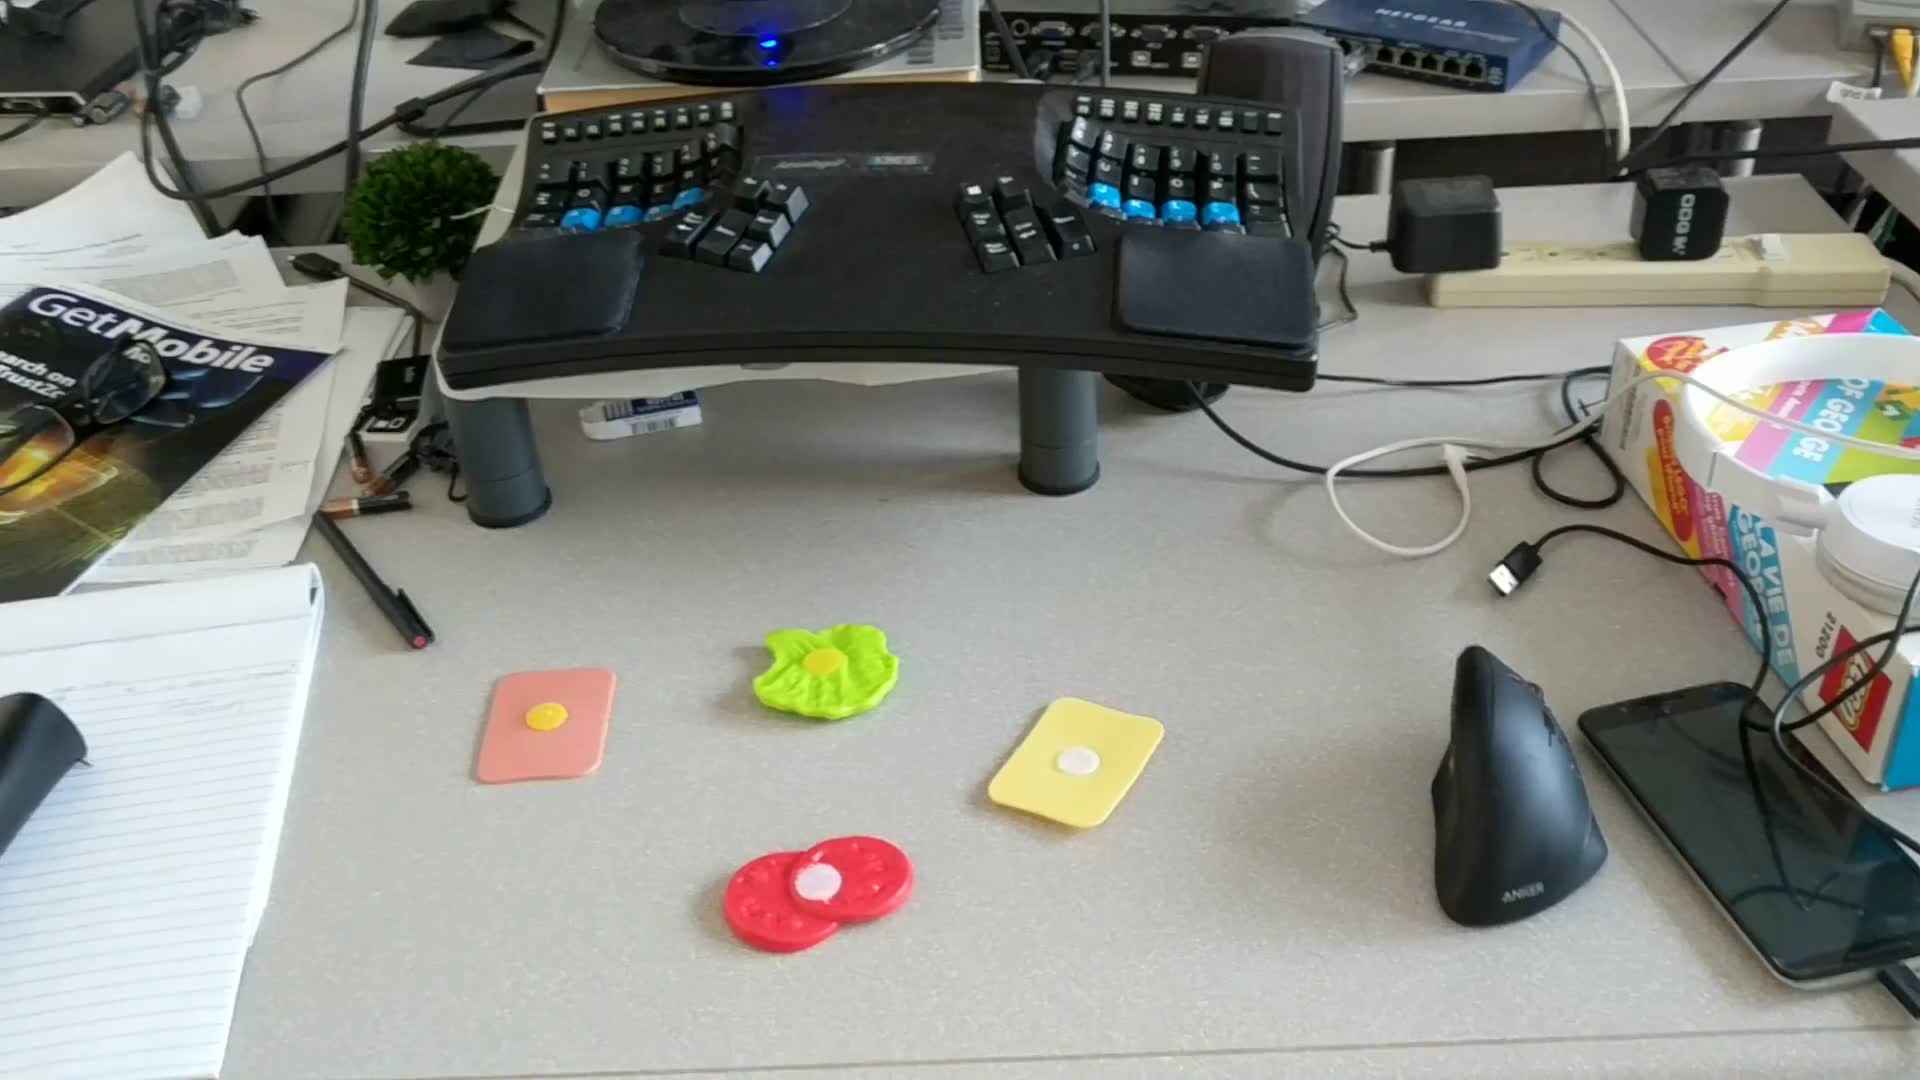
\includegraphics[width=\textwidth]{FIGS/sandwich-training-1.jpg}
  \end{minipage}
  \begin{minipage}[b]{0.32\textwidth}
    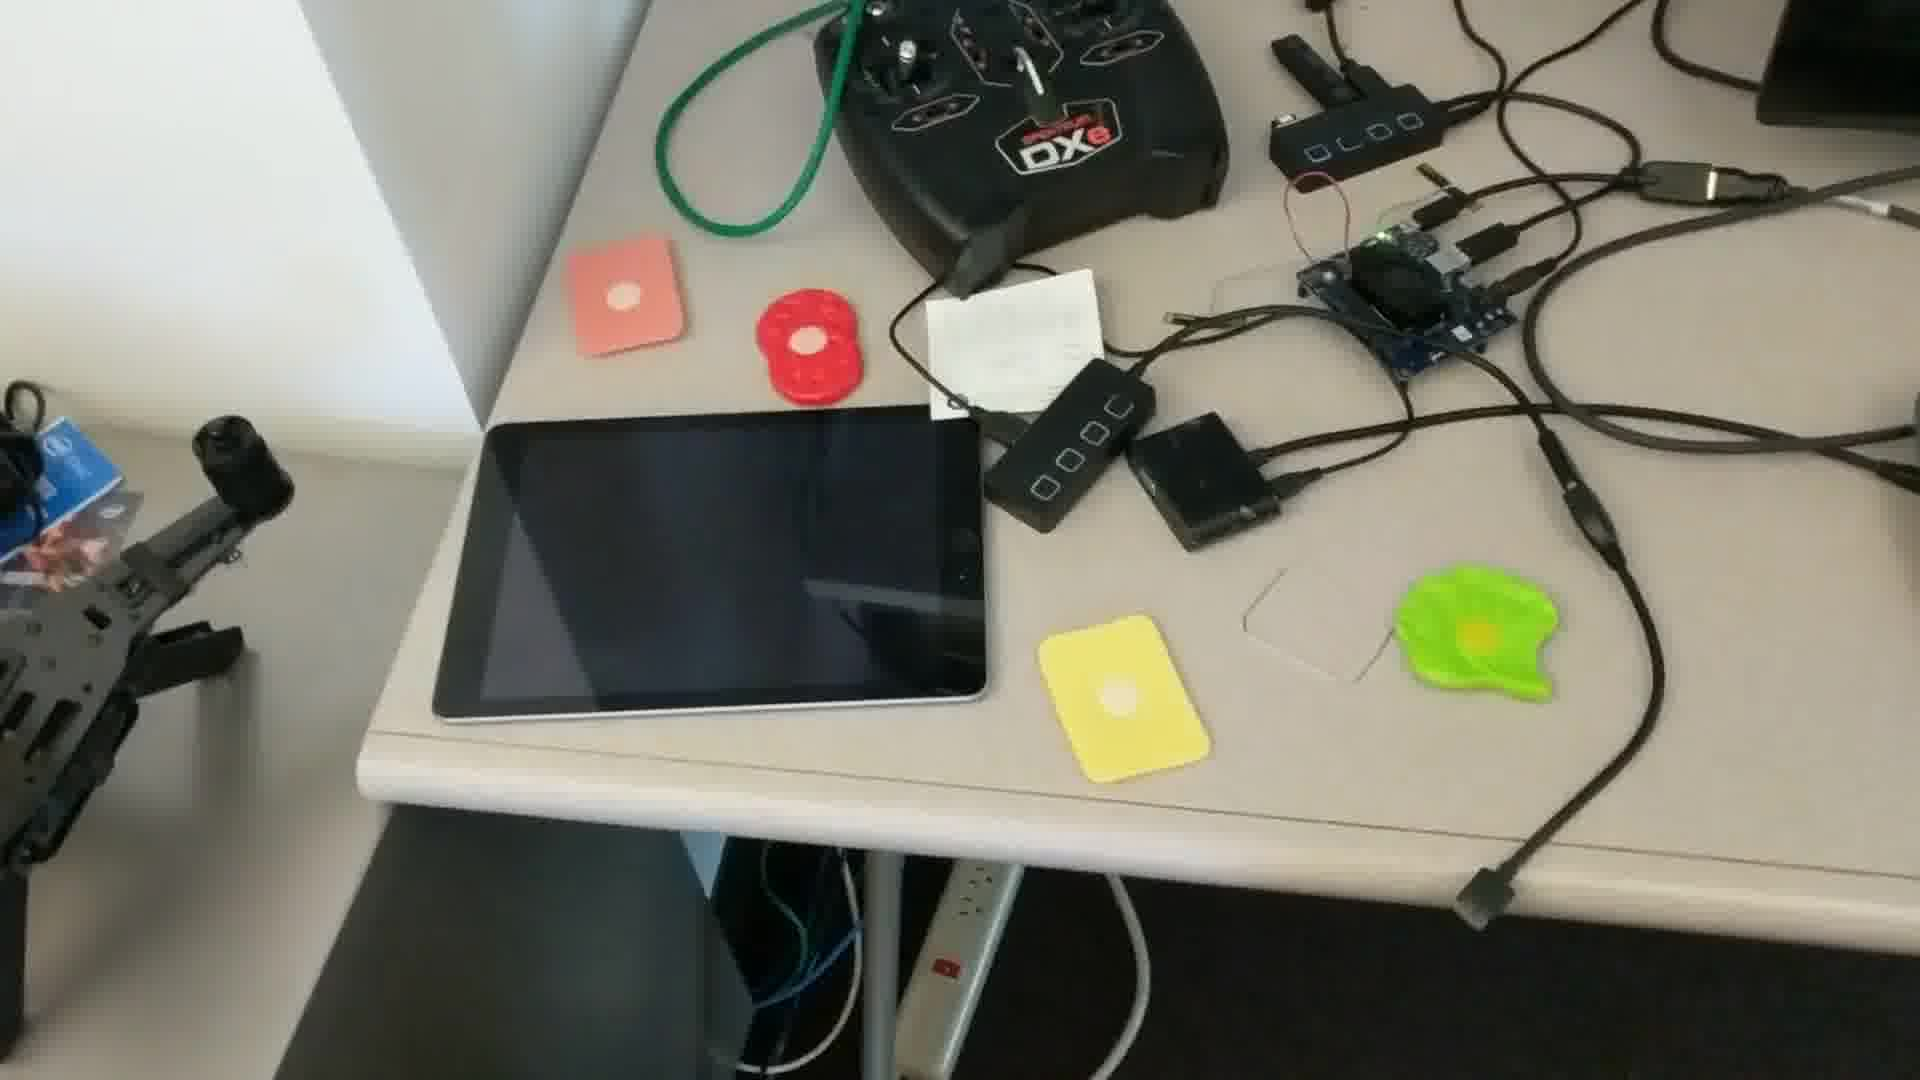
\includegraphics[width=\textwidth]{FIGS/sandwich-training-2.jpg}
  \end{minipage}
  \begin{minipage}[b]{0.32\textwidth}
    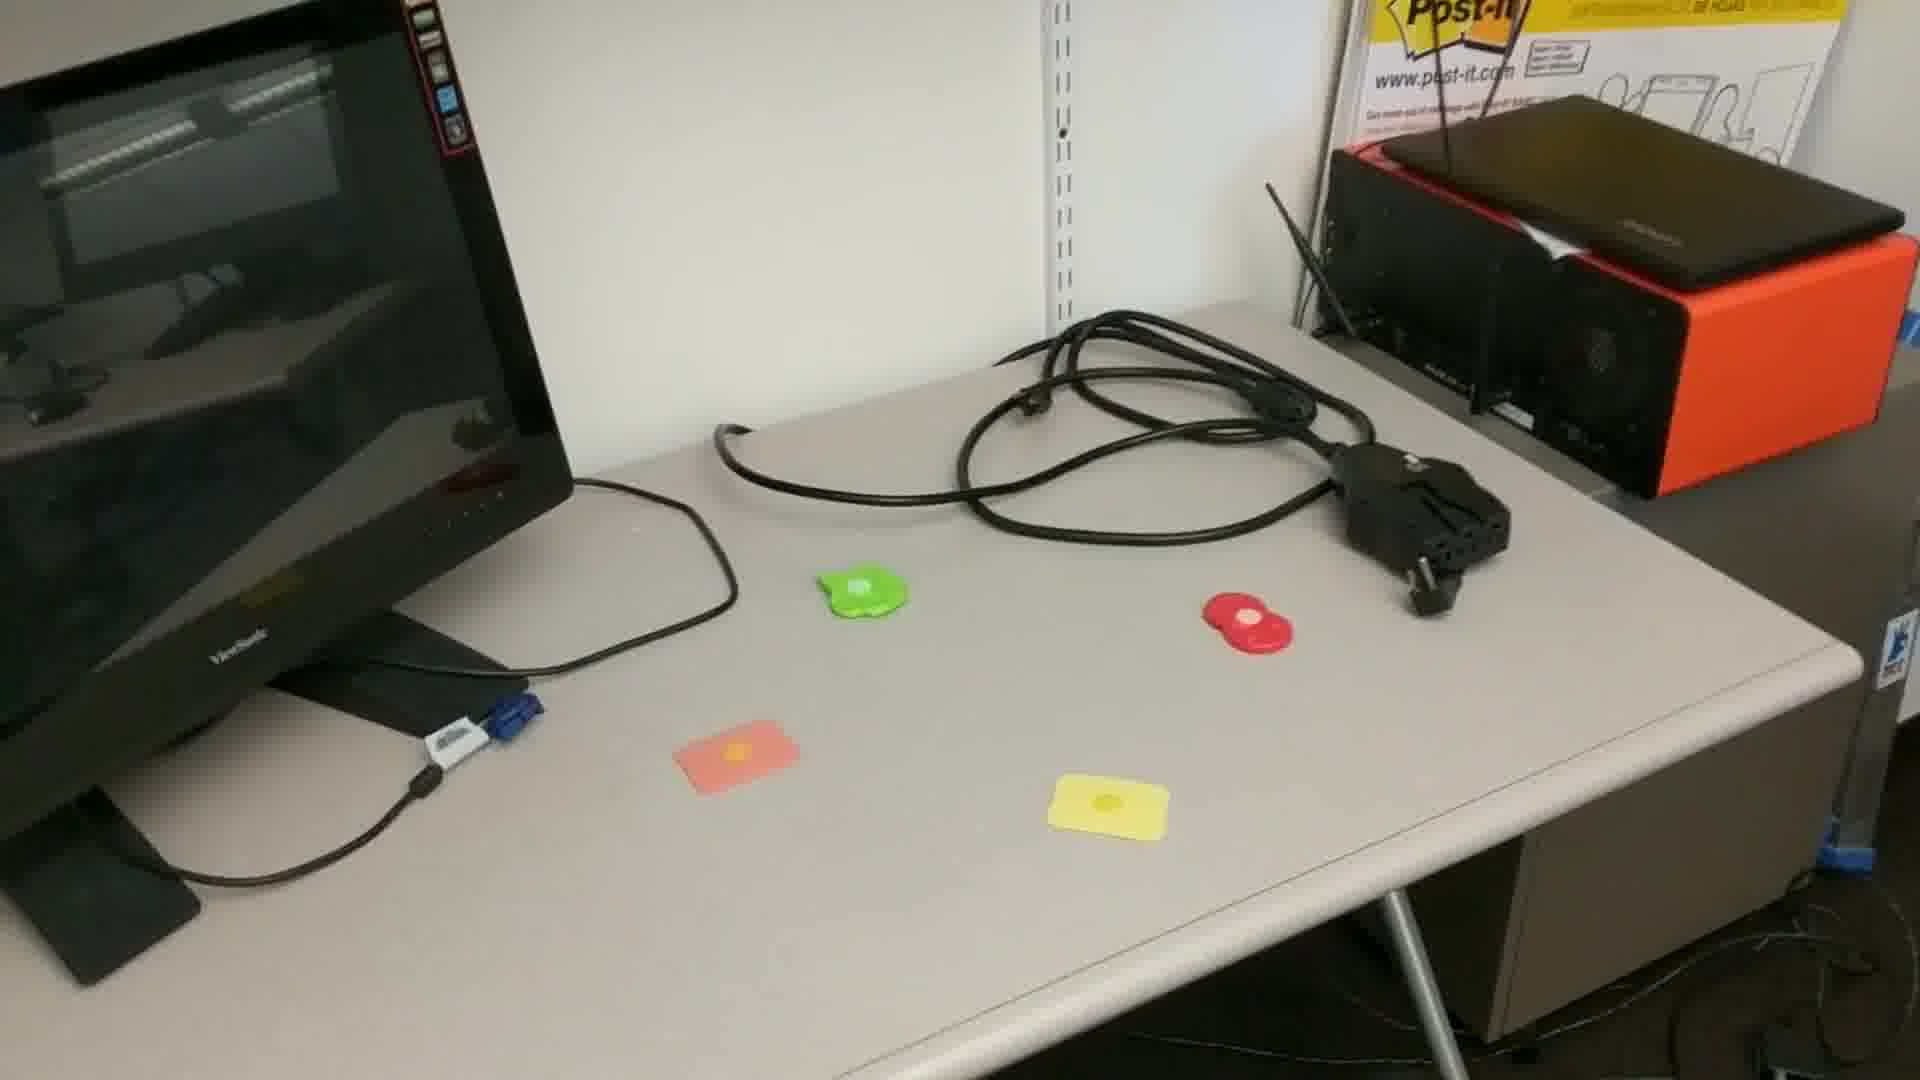
\includegraphics[width=\textwidth]{FIGS/sandwich-training-3.jpg}
  \end{minipage}
    \caption{OpenTPOD Training Images Examples}
  \label{figs:tpod-example-training-images}
\end{figure}

Using OpenTPOD to create object detectors is straight-forward. A developer first
captures videos of objects from various viewing angles and diverse backgrounds.
For example, these videos can be acquired on a mobile phone. At 30 frames per
second, ten minutes of video footage contain 18000 frames, which is already a
reasonable amount of training data for transfer learning. Larger amounts of
training data typically help increase the accuracy, although diminishing returns
apply. Moreover, it is preferred to collect training examples in environment
similar to the test environment to make the training examples exhibit similar
distribution as test data. Figure~\ref{figs:tpod-example-training-images} shows
three example training images for a toy cooking set. Note that the image
background is randomly cropped to be used as negative examples. These
background examples illustrate to the neural network what an object of interest
does \textit{not} look like. Therefore, it is recommended that the background contains
common objects in the test environment that may cause confusion.


\begin{figure}[]
  \centering
    \fbox{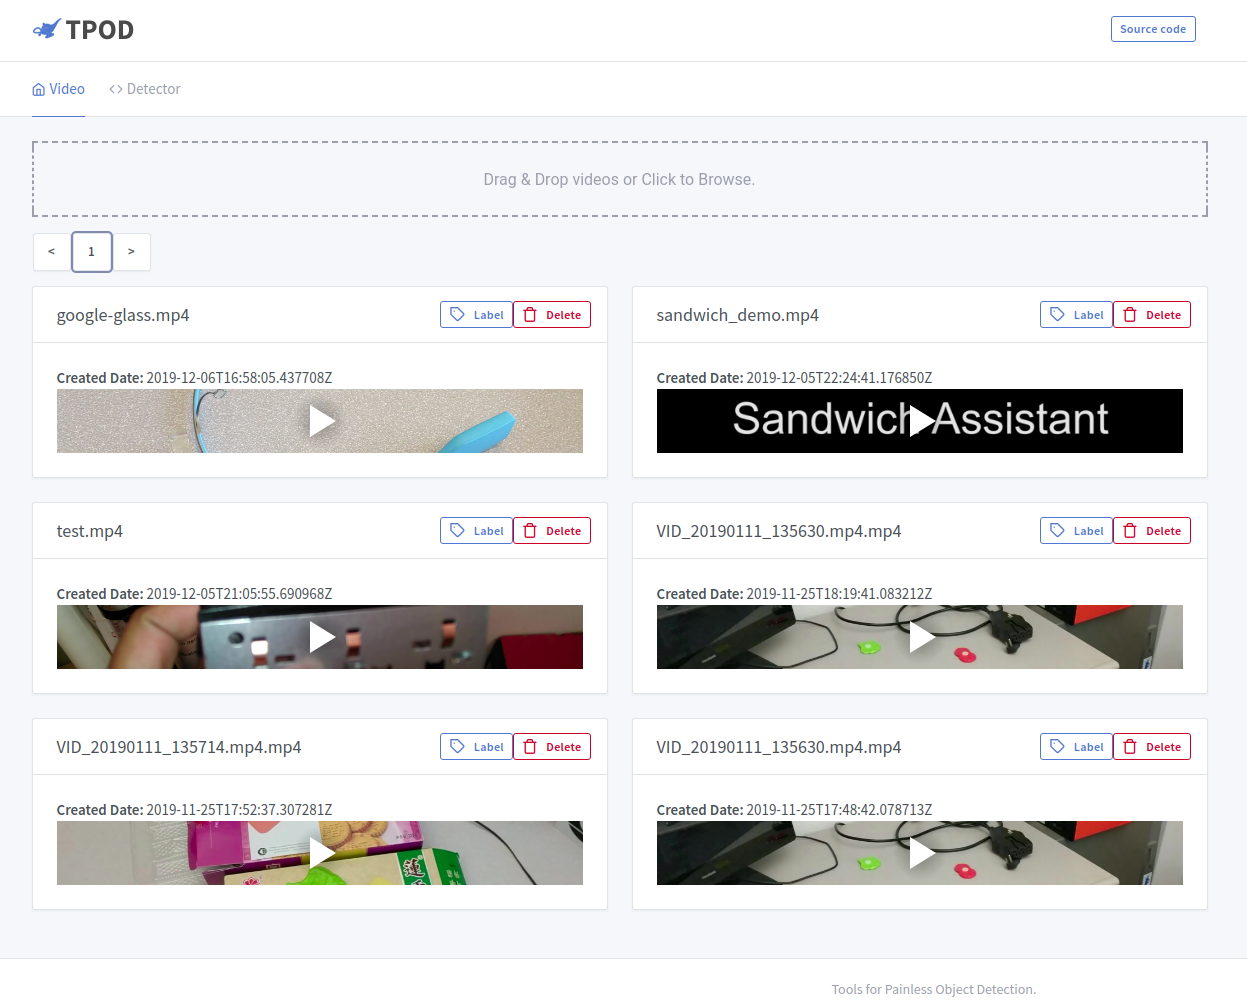
\includegraphics[width=\textwidth]{FIGS/tpod-video-gui}}
    \caption{OpenTPOD Video Management GUI}
  \label{figs:tpod-video-gui}
\end{figure}

Next, developers upload the collected training videos to OpenTPOD either directly
from the phone or from a computer. As shown in Figure~\ref{figs:tpod-video-gui},
OpenTPOD helps user to store and organize training videos. In addition, OpenTPOD assists
users to annotate the training videos by integrating an external labeling tool
into the GUI. Uers can annotate objects by draw bounding boxes on the uploaded
video frames. To facilitate the annotation process, OpenTPOD leverages the fact that
the individual frames come from a continuous video shoot. It automatically
generates bounding box in subsequent frames either using a correlation tracking
algorithm~\cite{danelljan2014accurate} or linear interpolation. As a result,
users only need to label a few key frames in a video with the rest of frames
auto-populated with generated labels. Of course, tracking is not perfect, and
the bounding box may drift off over time. In this case, the user can forward or
rewind the video to adjust the bounding box.  The adjustment of bounding boxes
re-initializes the tracking for subsequent frames. From our experience usage,
this approach of labeling followed by tracking can reduce the number of frames
that the user needs to manually label by a factor of 10-20x.

\begin{figure}[]
  \centering
    \fbox{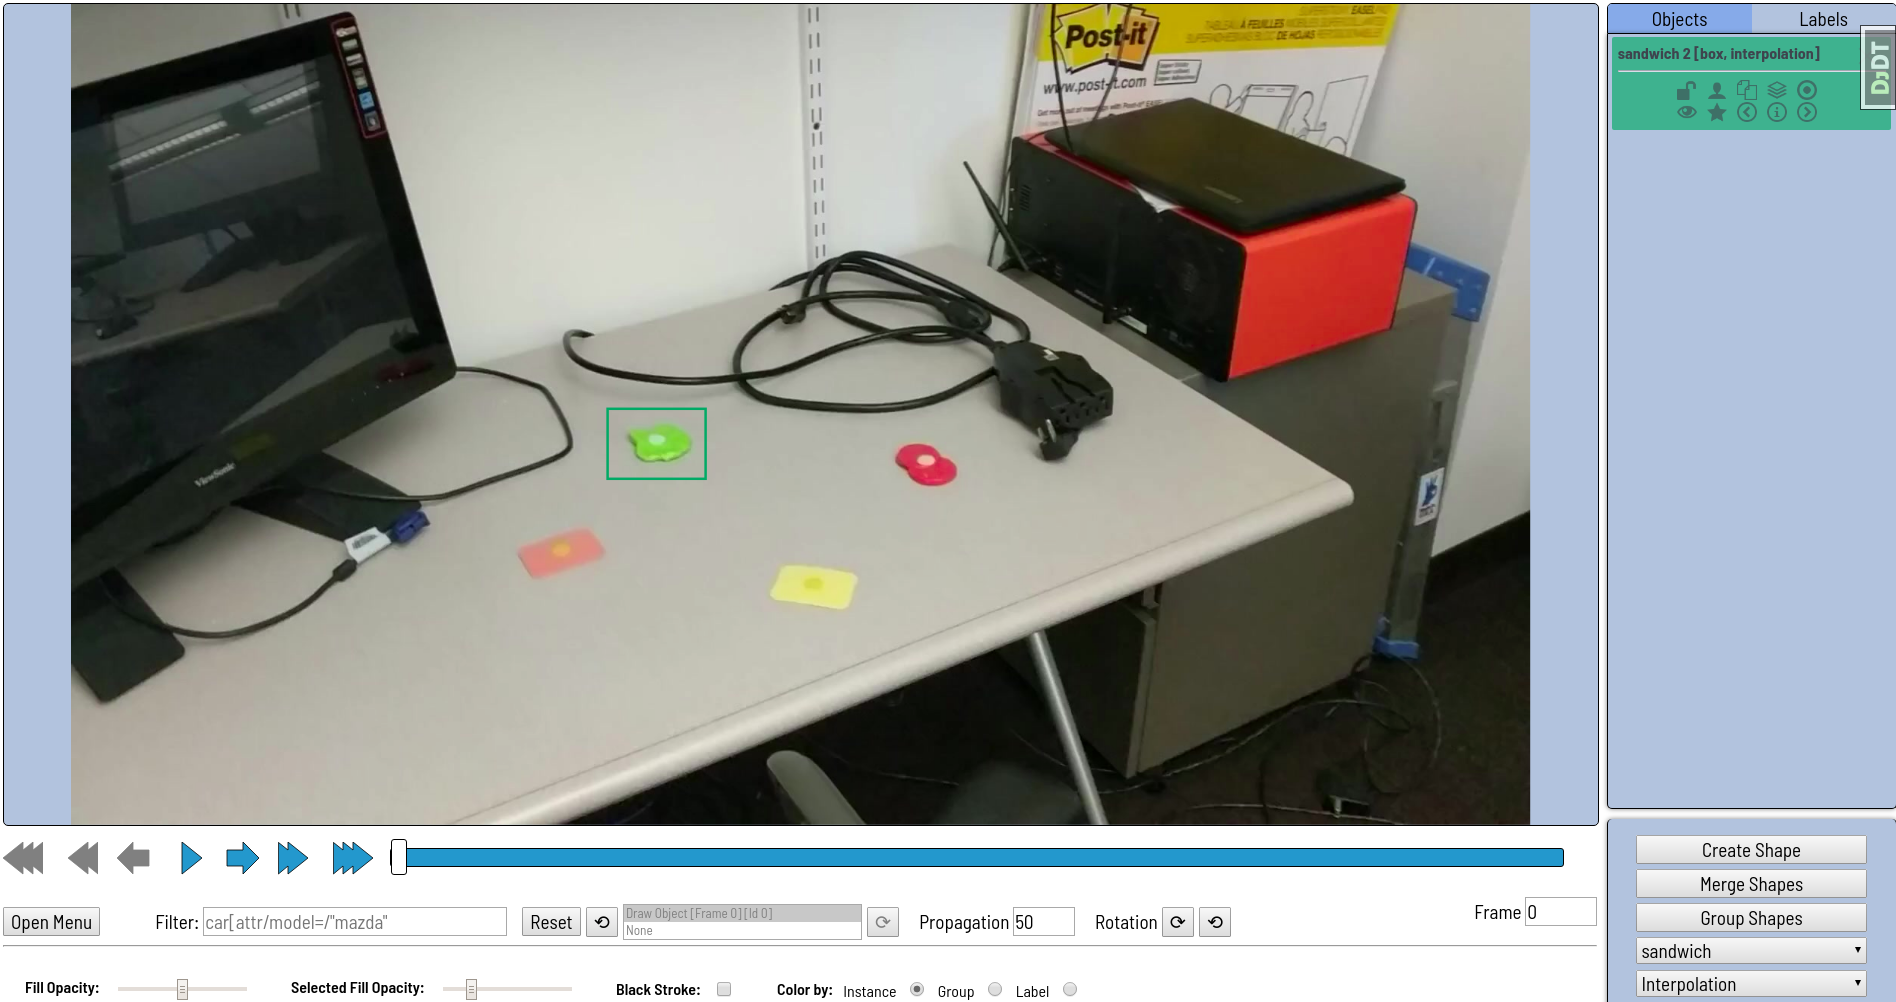
\includegraphics[width=\textwidth]{FIGS/tpod-label-gui}}
    \caption{OpenTPOD Integration of an External Labeling Tool}
  \label{figs:tpod-label-gui}
\end{figure}

With videos annotated, users can move on to create a training dataset on the
webpage by selecting videos to use. OpenTPOD performs a data cleaning and
augmentation pass to prepare a high quality training set. Due to inter-frame
correlation, adjacent frames within a video may appear to be substantially
similar or identical. These highly correlated frames violate the independent and
identically distributed assumption of training data for DNNs. OpenTPOD eliminates
these near duplicate examples. Optionally, data augmentation can be employed. It
adds synthetic images, created by cutting and pasting the object of interests on
varying backgrounds, at different scales and rotations. Such augmentation helps
produce more robust object detectors~\cite{dwibedi2017cut}.

Then, by submitting a form on the web GUI, users can launch the DNN training
process without writing a single line of code. Under the hood, OpenTPOD automates
the transfer learning process. OpenTPOD supports several state-of-the-art object
detection networks, including FasterRCNN-ResNet~\cite{ren2015faster,He2016} and
SSD-MobileNet~\cite{Liu2016,Howard2017}. These different networks exhibit
varying accuracy versus speed trade-offs. While FasterRCNN-ResNet achieves higher
accuracies on standard datasets, its training and inference time are
significantly longer than SSD-MobileNet. Application developers should choose
the appropriate DNN network based on their accuracy and latency constraints.
Negative examples are mined from the video background; these are parts of the
frames not included in the object bounding boxes.  The training process
generates downloadable Tensorflow models in the end. The OpenTPOD web GUI provides
training monitoring through Tensorflow visualization library
Tensorboard~\cite{tensorflow2017}. OpenTPOD also provides a container image that can
serve the downloaded model files for inference.

Overall, OpenTPOD can greatly reduce both the labeling effort and in-depth
machine learning knowledge required to train and deploy a DNN-based detector.
The OpenTPOD demo video can be found at \url{https://youtu.be/UHnNLrD6jTo}.
OpenTPOD has been used by tens of researchers and students to build wearable
cognitive assistance. For example, a group of master students in CMU mobile and
pervasive computing class successfully used OpenTPOD to build an assistant for
using Automated External Defibrillator (AED) machines.

\subsection{OpenTPOD Case Study With the COOKING Application}

To quantify how much OpenTPOD can help reduce labeling efforts, we conducted a case
study to train detectors for the COOKING cognitive
assistant~\cite{chen2018application}. We trained object detectors for 9
components of a toy sandwich, including bread, ham, lettuce, cucumber, cheese,
half sandwich, wrong ham, tomato, and full sandwich. We collected 53 short
training videos, annotated all of them, and trained object detectors with OpenTPOD.

In total, we collected 21218 video frames. In contrast, we only manually labeled
91 frames on OpenTPOD annotation interface. The rest of frames are automatically
labeled by tracking. The entire labeling session took 80 minutes. The total
number of frames used for training is 21013 due to training set optimization by
OpenTPOD. We fine-tuned from a FasterRCNN-VGG network. The transfer learning process
took 54 minutes to finish on a NVIDIA K40c GPU.


\subsection{OpenTPOD Architecture}

\begin{figure}[]
  \hspace{-.1in}
    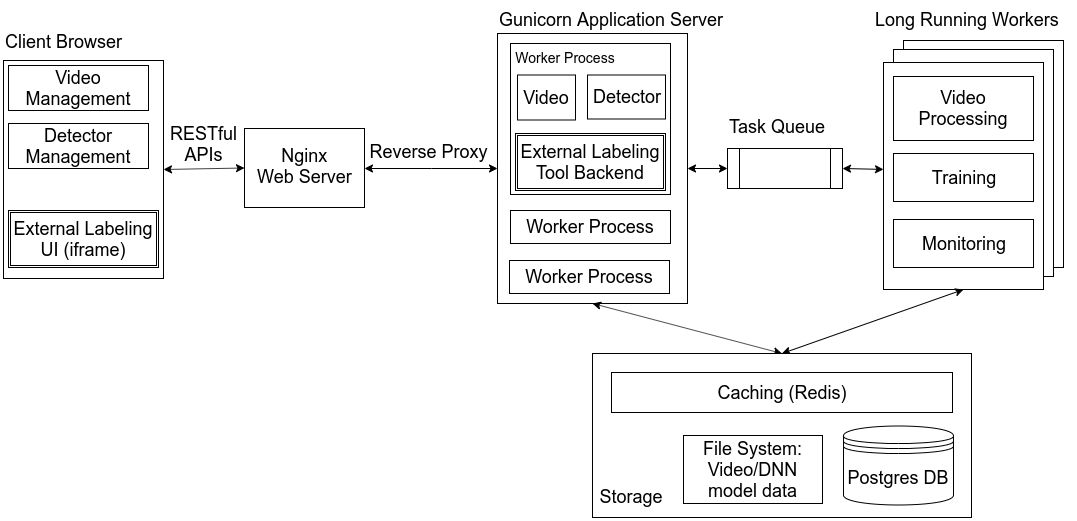
\includegraphics[width=1.1\textwidth]{FIGS/tpod-arch}
    \caption{OpenTPOD Architecture}
  \label{figs:tpod-arch}
\end{figure}

OpenTPOD adopts a Model-View-Controller (MVC) design~\cite{krasner1988description}.
Figure~\ref{figs:tpod-arch} shows the OpenTPOD architecture. The OpenTPOD frontend
handles UI logic and is built using React, a declarative, efficient, and
flexible JavaScript library for creating user interfaces~\cite{staff2016react}.
React enables OpenTPOD frontend code to be modular and reusable. The frontend has
three major components: video management, detector management, and an external
labeling tool. OpenTPOD integrates the labeling tool CVAT~\cite{cvat2019} into its
frontend UI through HTML iframe embedding. The integration of an labeling tool
into the OpenTPOD GUI unifies the workflow. Users no longer need to install and set
up another piece of software. The OpenTPOD frontend communicates with the backend
through a set of RESTful APIs~\cite{richardson2008restful}. 

OpenTPOD backend is developed using the Django web
framework~\cite{holovaty2009definitive} and served with the Nginx web
server~\cite{nedelcu2010nginx} and the Gunicorn gateway~\cite{gunicorn2017http}.
The backend implements RESTful apis to create, read, update, and delete
\textit{Video} and \textit{Detector} resources. It also interfaces with the
backend of the external labeling tool to read and write annotations. Long
running background jobs, such as DNN model training and video extraction, are
processed asynchronously using a task queue and worker processes. Metadata about
videos and DNN models are stored in a relational database while large binary
files, such as video files and trained DNN model weights, are stored in the file
system. An in-memory caching layer on top of the file system and database is
created using the Redis key-value store. The entire application is containerized and
can be deployed easily onto bare-metal or virtualized environments.

One key design choice of OpenTPOD is to be extensible for new DNN architectures.
OpenTPOD provides a standard interface, shown in
Figure~\ref{figs:tpod-provider-interface}, in order to easily add new DNNs
implementation for transfer learning. OpenTPOD refers to these DNN implementations
as DNN \textit{Providers}. Without modifying other components, providers can be
added and integrated by implement this interface. The built-in \textit{Provider}
is the Tensorflow Object Detection API~\cite{tfod2019}, which supports transfer
learning for a wide set of object detectors. 


\begin{algorithm} 
% \addcontentsline{OpenTPOD Provider Interface}{algorithm}{OpenTPOD Provider Interface}
\SetAlgoLined
 property \textbf{training\_configurations}: user customizable hyperparameters\;
 \textbf{init(dnn\_type, training\_set, output\_directory)}: initialization\;
 \textbf{train(training\_configurations)}: launch training\;
 \textbf{export()}: export trained models\;
 \textbf{visualization()}: monitor training process\;
\caption{OpenTPOD Provider Interface}
\label{figs:tpod-provider-interface}
\end{algorithm}